% ==============================================================================
%  styles/settings.tex —— 全局导言、字体、标题、页眉页脚
%  由 main.tex 载入；主题配色在 palettes/themes.tex 中覆盖
% ==============================================================================

% ---------------- 宏包 ----------------
\usepackage[textwidth=17cm,top=2.3cm,bottom=2cm]{geometry}
\usepackage{amsmath}
\usepackage{amsthm}
\usepackage{amsfonts}
\usepackage{amssymb}
\usepackage{tikz}
\usepackage{xcolor}
\usepackage[most]{tcolorbox}
\usepackage{graphicx}
\graphicspath{{assets/pdf/}{assets/tikz/}}
\usepackage{fontspec}
\usepackage{enumitem}
\usepackage{multicol}
\usepackage{tocloft}
\usepackage[explicit]{titlesec}
\usepackage{atbegshi}
\usepackage{changepage}
\usepackage{setspace}
\usepackage{adjustbox}
\usepackage{calc}
\usepackage{subcaption}
\usepackage[hidelinks]{hyperref}% 去掉链接边框（hidelinks）
\usetikzlibrary{calc}
\tcbuselibrary{skins, theorems}

% ---------------- 默认配色（可被 palettes/themes.tex 覆盖） ----------------
\definecolor{lv}{RGB}{131, 187, 170}       % 绿色
\definecolor{huang}{RGB}{227, 164, 60}     % 黄色
\definecolor{hong}{RGB}{149, 44, 38}       % 红色

\definecolor{qiancheng}{RGB}{227, 101, 53} % 橙色
\definecolor{heise}{RGB}{0,0,0}            % 黑色
\definecolor{mibai}{RGB}{244, 237, 218}    % 米白色
\definecolor{qianbai}{RGB}{248, 243, 231}  % 浅白色

\definecolor{definition}{RGB}{245,164,0}
\definecolor{theorem}{RGB}{222,4,20}
\definecolor{proposition}{RGB}{177,0,129}
\definecolor{corollary}{RGB}{133,194,72}
\definecolor{lemma}{RGB}{233,93,157}
\definecolor{example}{RGB}{0,153,216}

% ---------------- 字体 ----------------
\newcommand{\AvantGarde}{%
	\fontspec[
	Path = ./assets/fonts/,
	Extension = .otf,
	UprightFont = *
	]{ITC Avant Garde Gothic Bold}%
}

\newcommand{\SiYuan}{%
	\fontspec[
	Path = ./assets/fonts/,
	Extension = .otf,
	UprightFont = *
	]{SiYuan}%
}

% ---------------- 标题格式 ----------------
% 一级标题
\titleformat{\section}{
	\centering
	\fontsize{24pt}{18pt}\selectfont\SiYuan\XeTeXinterchartokenstate=0
	\color{qiancheng}
}{}{0pt}{#1}

\titlespacing*{\section}
{0em}
{1.5em plus 1em minus .2em}
{1em}

% 二级标题样式在 styles/boxes.tex 中由 \TitleBoxI 统一接管

% ---------------- 页眉页脚 ----------------
\AtBeginShipout{%
	\AtBeginShipoutAddToBox{%
		\begin{tikzpicture}[remember picture, overlay]
			\node[    % 左页眉
			anchor=north west,
			font=\fontsize{20pt}{12pt}\bfseries\SiYuan,
			text=mibai,
			inner sep=10pt
			] at ($(current page.north west) + (30pt, 0pt)$) {
				{\XeTeXinterchartokenstate=0 \leftmark}
			};
			\node[    % 右页眉
			anchor=north east,
			font=\fontsize{20pt}{12pt}\bfseries\SiYuan,
			text=mibai,
			inner sep=10pt
			] at ($(current page.north east)+(-5pt,0pt)$) {
				{\XeTeXinterchartokenstate=0 \rightmark}
			};
			\node[    % 页码
			anchor=south west,
			font=\fontsize{12pt}{12pt}\bfseries\AvantGarde,
			text=mibai,
			align=center,
			minimum width=60pt,
			minimum height=20pt
			] at ($(current page.south west) + (268.5pt, 20pt)$) {
				\thepage
			};
		\end{tikzpicture}%
	}%
}

% ---------------- 正文格式 ----------------
\setstretch{1.5}
\parindent=2em
\parskip=0pt

% ---------------- 正文背景 ----------------
% 全幅科技满铺背景。
% 性能：背景图只在第一页以真实尺寸嵌入一次，之后通过 PDF 的 XObject
% 复用机制重复引用，避免每页各嵌一份 174KB 的图。
\newbox\LoneBgBox
\newcommand{\DrawLoneTrailBackground}{%
	\AddToHook{shipout/background}{%
		\begin{tikzpicture}[remember picture, overlay]
			\node[anchor=north west, inner sep=0pt, outer sep=0pt]
			at (current page.north west) {%
				\ifvoid\LoneBgBox
					\global\setbox\LoneBgBox\hbox{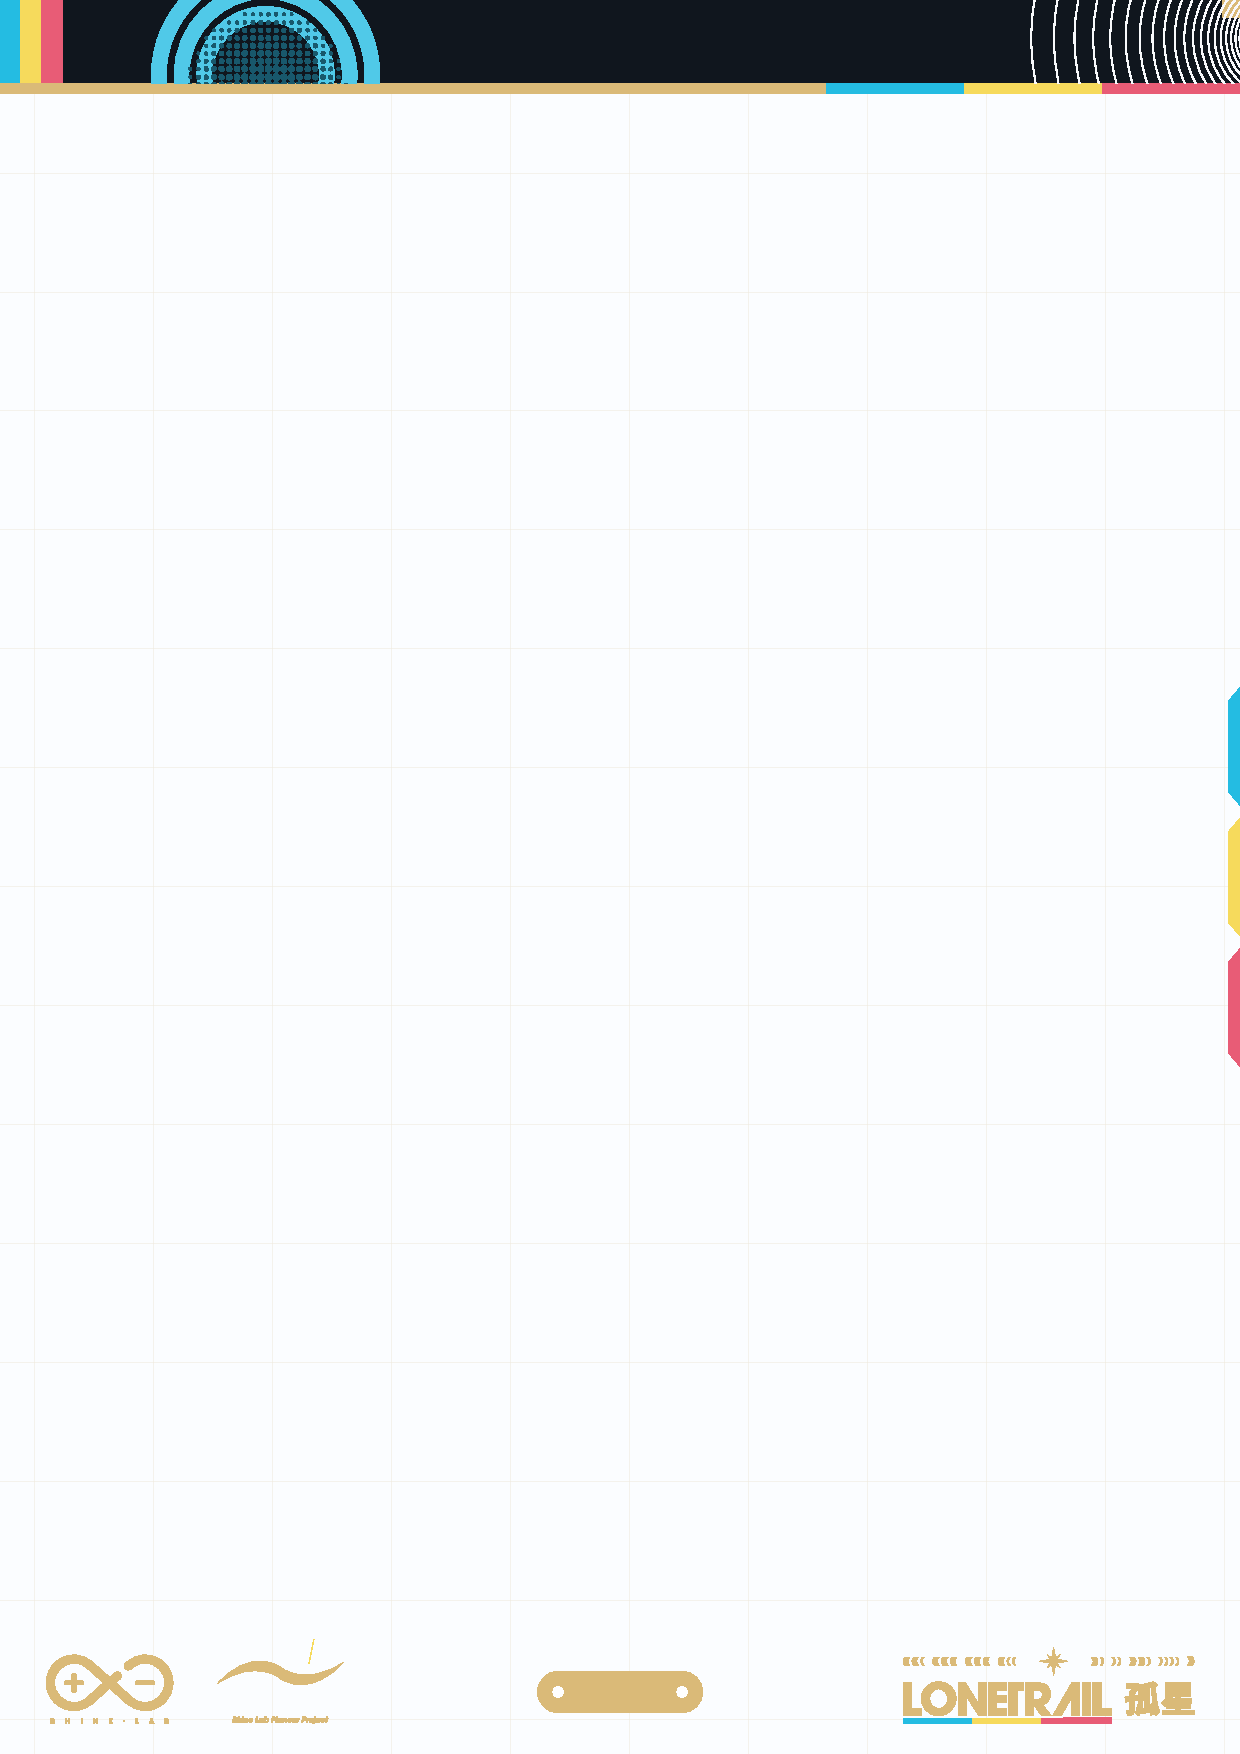
\includegraphics{assets/pdf/main_bg.pdf}}%
				\fi
				\resizebox{\paperwidth}{\paperheight}{\usebox\LoneBgBox}%
			};
		\end{tikzpicture}%
	}%
}
